We used a number of tests to validate the code. 


\section{Multigroup Scattering, No Upscatter}
To test the Gauss-Seidel multigroup scattering method we use the two group diffusion equation as a benchmark. 
\begin{align}
 D_1\nabla^2 \phi_1 - \Sigma_{r, 1 \rightarrow 1} \phi_1 + s_1^{'''} &= 0 \\
 D_2\nabla^2 \phi_2 - \Sigma_{r, 2 \rightarrow 2} \phi_2 + s_2^{'''} + \Sigma_{s, 1 \rightarrow 2} \phi_1 &= 0
\end{align}

where $D_g = \frac{1}{3\Sigma_{t, g}}$ and $\Sigma_{r, g \rightarrow g} = \Sigma_{t, g} - \Sigma_{s, g \rightarrow g}$. In an infinite medium we can assume no gradient, so the flux should approach $\frac{s_1^{'''}}{\Sigma_{r, 1}}$ in the first energy group and $\frac{s_2^{'''} + \phi_1 \Sigma_{s, 1 \rightarrow 2}}{\Sigma_{r, 2}}$ in the second.  

This problem was run with $ s^{'''} = 1$ for both groups, $\Sigma_{s, 1\rightarrow 2} = 11$, $\Sigma_{r, 1} = 2$ and $\Sigma_{r, 2} = 1$ This gives an expected flux of $0.50 $ in the first group and $1.50$ in the second. 

\section{NDA/SAAF Agreement}
As the SAAF equation is non-conservative, its solution does not necessarily agree with the low order equation it is coupled with. However, the two solutions should approach each other as the number of mesh cells increases \cite{Wang2013}. Our code replicates this behavior. 
\begin{figure}
    \centering
    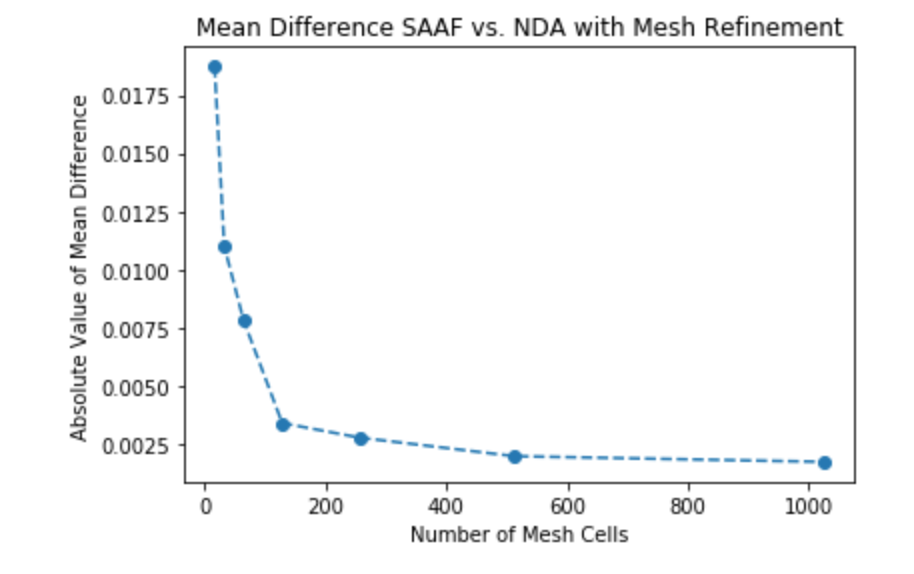
\includegraphics[width=.75\textwidth]{fig/SAAFvsNDA}
    \caption{SAAF/NDA Agreement with Mesh Refinement}
    \label{fig:SAAFvsNDA}
\end{figure}